\documentclass[thesis.tex]{subfiles}

\chapter{Tổng quan bài toán và đặt vấn đề}
\section{Giới thiệu bài toán}
Bài toán mà chúng ta cần giải quyết ở đây như sau:
\begin{itemize}
	\item Đầu vào: Ảnh chụp đường phố từ tập dữ liệu Cityscapes không nhãn trong lúc huấn luyện 
	\item Đầu ra: Kết quả phân vùng ngữ nghĩa với 19 lớp bao gồm:
	
	road-lòng đường; sidewalk-vỉa hè; building-toà nhà; wall-bức tường; fence-hàng rào
	
	pole-cột; light-đèn; sign-biển báo; vegetation-cây cối; terrain-địa hình
	
	sky-bầu trời; person-người; rider-người đạp xe; car-xe hơi; truck-xe tải
	
	bus-xe buýt; train-đoàn tàu; motorcycle-xe máy; bicycle-xe đạp
\end{itemize}

Bài toán phân vùng ảnh ngữ nghĩa bán giám sát là một bài toán quan trọng, bao gồm nhiều bài toán con khác nhau như: bài toán phân vùng ngữ nghĩa, bài toán thích ứng miền, bài toán học cạnh tranh. Đây là một bài toán phức tạp và đòi hỏi độ chính xác cao bởi vì các thông tin trong ảnh đường phố khá đa dạng và phức tạp bao gồm nhiều lớp, nhiều thông tin cần xử lý. Hơn nữa, bài toán học bán giám sát còn khó khăn hơn khi mô hình không được tiếp cận trức tiếp với nhãn của ảnh mà phải thích nghi qua một tập dữ liệu khác gần tương tự mà ta sẽ trình bày ở phần sau.

\section{Phân vùng ngữ nghĩa}
 
Phân vùng ngữ nghĩa là một nhiệm vụ nhằm phân loại từng điểm ảnh trong 1 ảnh từ một tập các lớp được định nghĩa trước. Hay đơn giản có thể hiểu đó là việc phân loại các đối tượng trong một ảnh vào các lớp đã định nghĩa trước đó.

Ví dụ như phân vùng ảnh để tìm con mèo hay con bò. Các lớp khác như bầu trời, cây, bãi cỏ được thể hiện trong Hình \ref{fig:semantic_segmentation}.

\begin{figure}[htp]
	\centering
	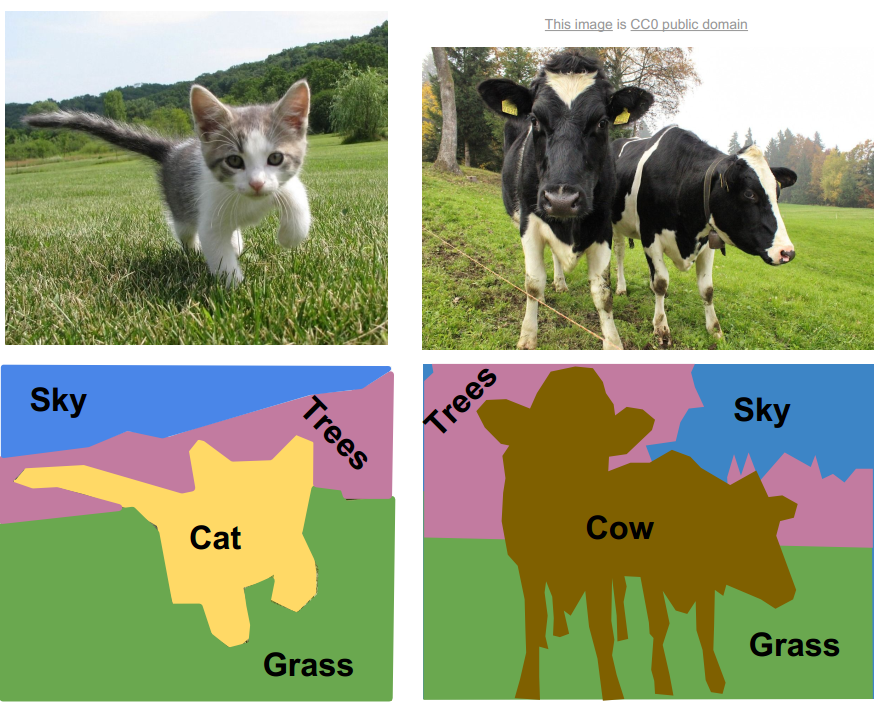
\includegraphics[width=0.6\textwidth]{images/semantic_segmentation.png}
	\caption{Một ví dụ của phân vùng ngữ nghĩa \protect\footnotemark}
	\label{fig:semantic_segmentation}
\end{figure}

Mục tiêu của lớp bài toán này là từ ảnh đầu vào với shape = (W, H, 3) để tạo ra ma trận WxH đầu ra với mỗi điểm ảnh sẽ là nhãn tương ứng được dự đoán. Ví dụ trong Hình \ref{fig:person-semantic-segmentation} ta phân vùng các nhãn là "Người", "Cái ví", "Cây/cỏ", "Toà nhà/Công trình". Từng điểm ảnh sẽ được phân vào một trong các nhãn được minh hoạ như hình bên phải

\begin{figure}[htp]
	\centering
	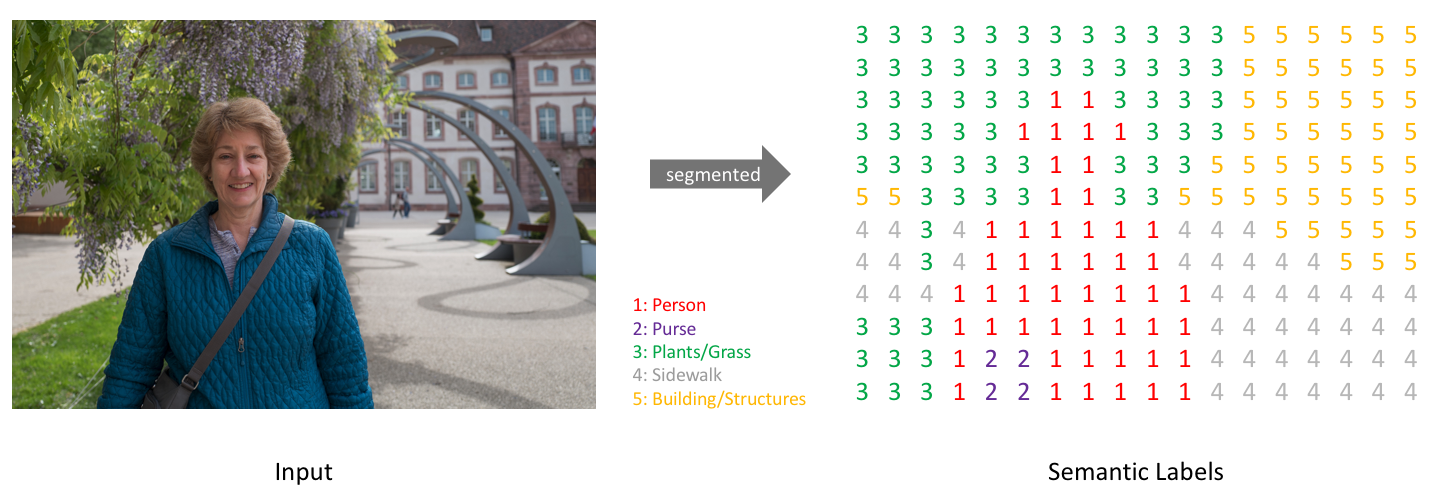
\includegraphics[width=0.7\textwidth]{person-semantic-segmentation.png}
	\caption{
		Minh hoạ cách một mô hình phân vùng ngữ nghĩa cho kết quả\protect\footnotemark}
	\label{fig:person-semantic-segmentation}
\end{figure}

Bài toán Phân vùng ngữ nghĩa khác với bài toán Phát hiện đối tượng ở chỗ nó sẽ không dự đoán "hình vuông bao quanh" đối tượng và cũng không phân biệt giữa các đối tượng khác nhau của một lớp (như với bài toán Phân vùng thực thể)

\begin{figure}[htp]
	\centering
	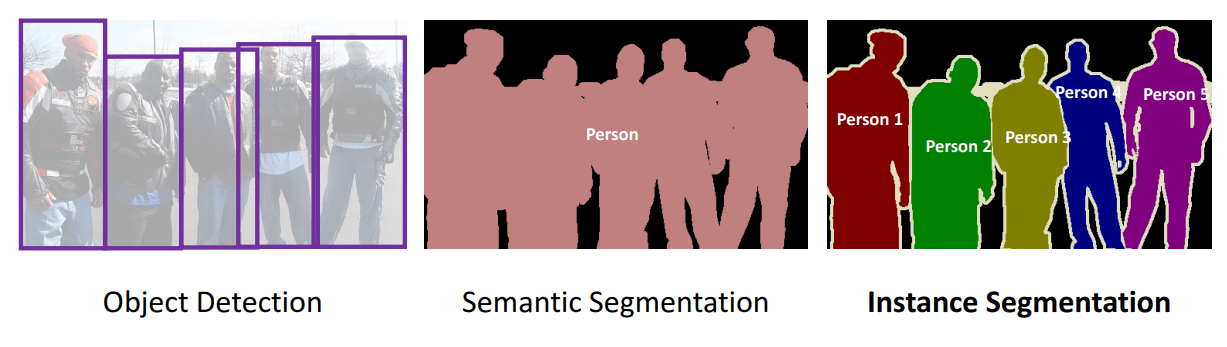
\includegraphics[width=0.7\textwidth]{images/sematic_vs_instance.png}
	\caption{
	Sự khác nhau giữa 3 bài toán Phát hiện đối tượng, Phân vùng ngữ nghĩa và Phân vùng thực thể 
		  \protect\footnotemark}
	\label{fig:sematic_vs_instance}
\end{figure}

\section{Thích ứng miền dữ liệu trong bài toán phân vùng ngữ nghĩa}
Thành công của bài toán phân vùng ngữ nghĩa trong những năm gần đây chủ yếu được thúc đẩy bởi một lượng lớn dữ liệu được gán nhãn có thể truy cập được. 

Tuy nhiên, thu thập một lượng lớn dữ liệu được gán nhãn cho việc huấn luyện là một tác vụ tốn kém. Gần đây, những tiến bộ trong đồ hoạ máy tính đã cung cấp thêm giải pháp thay thế cho việc gán nhãn thủ công đắt đỏ. 

Một ví dụ được thể hiện trong Hình \ref{fig:domain-adaptation-overview}.

\begin{figure}[htp]
	\centering
	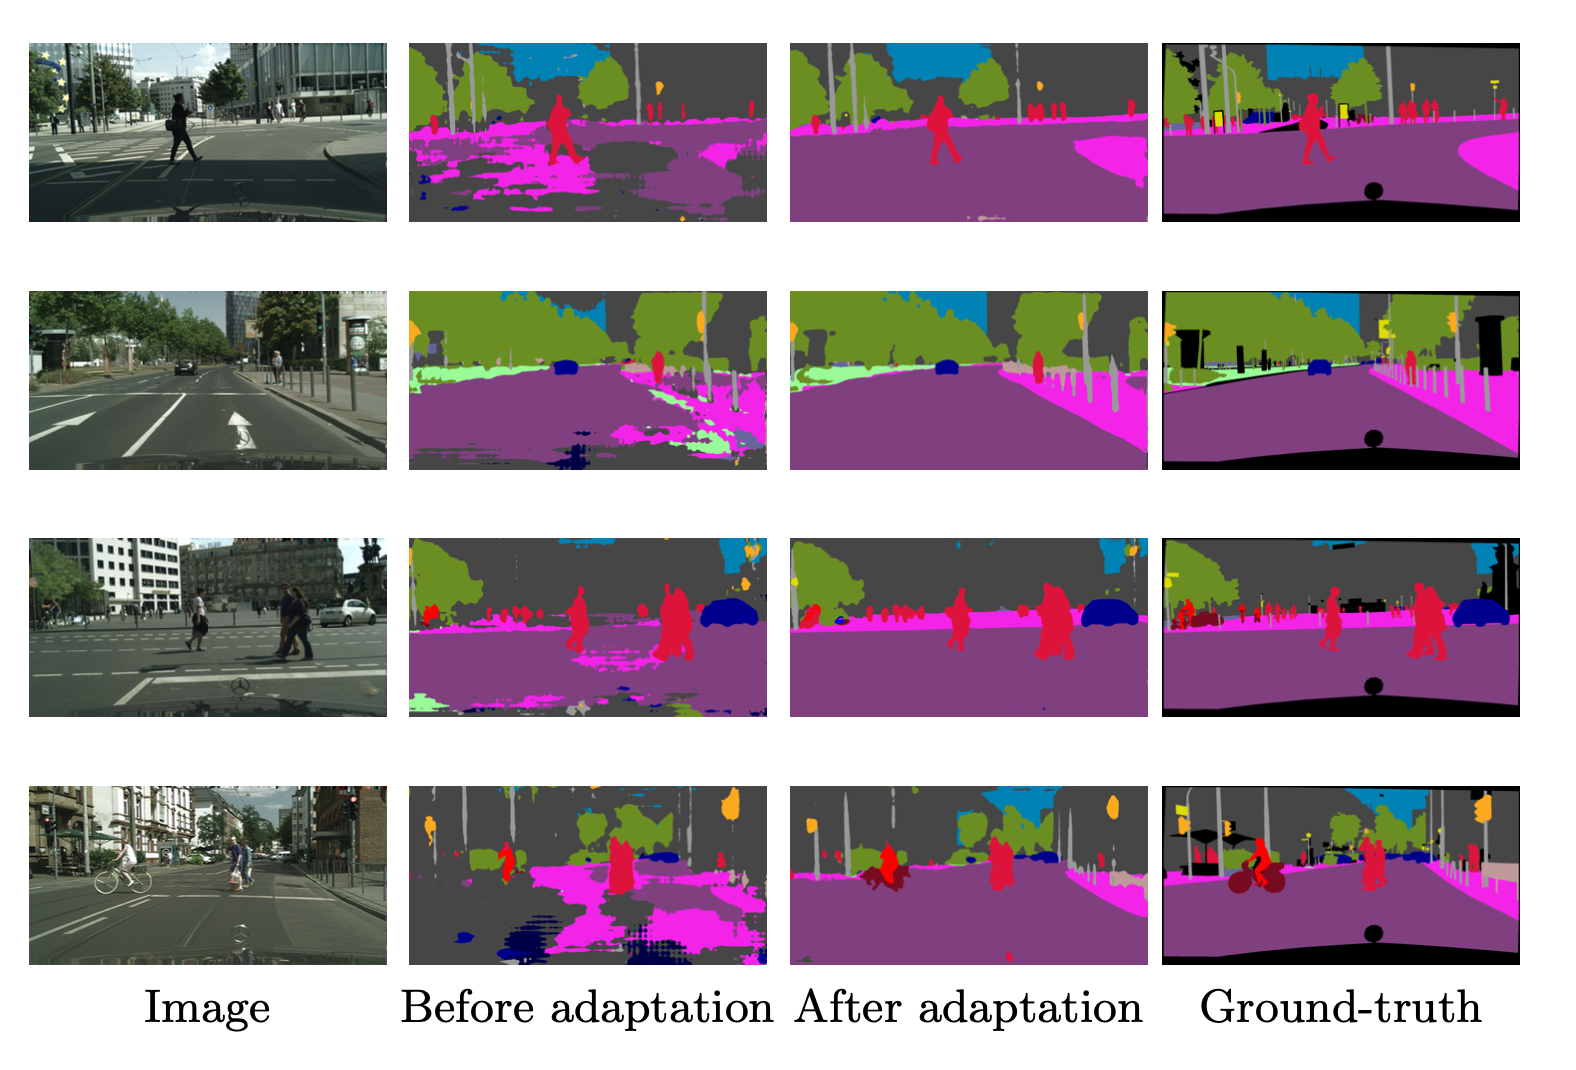
\includegraphics[width=1.0\textwidth]{images/domain-adaptation-overview.png}
	\caption{Một ví dụ của thích ứng miền\protect\footnotemark}
	\label{fig:domain-adaptation-overview}
\end{figure}

Gần đây, các phương pháp huấn luyện cạnh tranh (adversarial training - AT) đang nhận được nhiều sự quan tâm cho bài toán phân vùng ngữ nghĩa. Những phương pháp này nhằm tối ưu một chuỗi những hàm mục tiêu cạnh tranh để căn chỉnh các phân phối đặc trưng của tập đích và tập nguồn. Bên cạnh đó, một vài nghiên cứu khác tập trung vào xây dựng các mô hình dựa trên phương pháp tự huấn luyện (self-training - ST). Những phương pháp này đều lặp lại việc huấn luyện mô hình bằng cách sử dụng cả dữ liệu nguồn có nhẵn và nhãn giả được sinh ra cho dữ liệu đích, từ đó đạt được sự cân bằng giữa tập nguồn và tập đích. 

\section{Đóng góp của đồ án}
Trong kỷ nguyên công nghệ số như hiện nay, các sản phẩm mới, các kỹ thuật mới đang ngày ngày được sử dụng hoặc tích hợp, bổ sung cho các sản phẩm sẵn có trong sản xuất công nghiệp. Trong đó, lĩnh vực ô tô tự lái là một trong những mảnh đất màu mỡ cho các tập đoàn lớn và các nhà khoa học chinh phục. Có thể kể đến xe tự lái của Tesla (Hoa Kỳ) hay xa hơn có thể là sản phẩm xe tự lái của Vinfast (Việt Nam). Vậy làm sao để một chiếc xe có thể nhận dạng và phân tích các chướng ngại vật mà nó gặp phải trên đường ? 

Ta thấy rằng điều kiện làm việc của một chiếc ô tô là rất đa dạng về thời tiết, khí hậu, phong cảnh, ánh sáng, ... Để mô hình có thẻ hoạt động tốt thì đòi hỏi dữ liệu cũng phải đa dạng phù hợp với yêu cầu thực tế. Trong khi đó, để chuẩn bị dữ liệu ảnh đường phố thật đa dạng như vậy sẽ tốn kém chi phí và thời gian. Do đó, tác giả đã sinh dữ liệu ảnh đường phố từ trò chơi điện tử. Bên cạnh đó, ta không thể chỉ huấn luyện dữ liệu ảnh từ trò chơi rồi áp dụng vào ảnh thực tế được. Vậy nên, tác giả cần sử dụng thêm các kỹ thuật học máy nhằm tận dụng tốt dữ liệu. Tóm lại, đồ án này đóng góp một hướng tiếp cận với vấn đề trên bằng 2 tác vụ bao gồm: 

\begin{itemize}
	\item Sinh ảnh đường phố với các điều kiện thời tiết, ánh sáng, xe cộ, con người, ... khác nhau để cung cấp dữ liệu cho mô hình. 
	\item Áp dụng các kỹ thuật thích ứng miền và các mô hình cơ sở phù hợp với dữ liệu và yêu cầu bài toán nhằm tổng quát hoá khả năng nhận biết của mô hình.  
\end{itemize}